\section{Bornes de présentation Somfy}

\subsection{Somfy}

Somfy est une entreprise concevant des systèmes domotiques à l'attention du grand public.
Dans une démarche de communication, Somfy a contacté LTBL pour la création de 11 bornes interactives qui seront mises en place dans les magasins vendant les produits de la marque.

\subsection{Besoins}

L'objectif de ce projet est de concevoir et de produire 11 machines permettant d'afficher des informations sur l'entreprise et ses produits.
Ces informations peuvent être des vidéos, du texte ou des images.

Dans ce projet, je n'ai pas travaillé sur le développement de l'application de présentation, mais sur la mise en place des 11 machines permettant son exécution.
Ces 11 machines devaient présenter un système de visionnage pour réduire au maximum les possibilités de l'utilisateur.

\subsection{Recherches et choix du système}

Pour ce nouveau projet, j'ai proposé à mon maître de stage d'utiliser un système Linux pour l'exécution des applications sur les bornes.
Cela a pour avantage une plus grande flexibilité et capacité de customisation, mais aussi une gratuité de la licence.
En effet, il est simple de mettre en place un système captif sur une machine Linux, car on contrôle chaque élément de l'OS .

Pour le système, je me suis dirigé vers un membre de la famille Ubuntu pour sa stabilité et la grande communauté qui se forme autour.

J'ai alors découvert Ubuntu Core qui permet la création de systèmes embarqués et minimalistes.
Ubuntu Core est une variante d’ Ubuntu se basant sur des paquets unitaires séparés les uns des autres.
Cela permet de séparer chaque application et d'autoriser leur communication sur certains canaux particuliers appelés interfaces.
Ce système rappelle beaucoup les systèmes mobiles comme Android ou IOS exigeant des permissions définies à l'avance pour que les applications aient accès à certaines fonctionnalités.
Ubuntu Core utilise Snapcraft, un gestionnaire de paquet permettant cette séparation des applications.
De par sa complexité et de l'absence de serveur X sur SnapCraft, je n'ai pas retenu cette solution et me suis penché sur Ubuntu Server.

Ubuntu Server est une version d’ Ubuntu sans les composants de bureau classique.
Il permet de composer son propre système sans la lourdeur des applications graphiques inutiles dans le contexte des bornes Somfy.
J'ai donc choisi cette distribution ayant pour objectif d'installer un environnement de bureau manuellement.

\subsection{Environnement de kiosque}

Pour mettre en place l'environnement d'affichage, j'ai commencé par installer le serveur X .
Le serveur X est le logiciel en charge d'afficher l'interface à l'utilisateur au travers d'un protocole spécifique.

Après avoir installé ce logiciel, il faut installer un système de gestion de fenêtres qui sera en charge d'afficher les différentes fenêtres à la bonne taille et dans le bon contexte.
Pour le gestionnaire de fenêtres, j'ai choisi xfce, car il est léger et propose beaucoup de fonctionnalités.
Le gestionnaire de fenêtre est essentiel, car il permet aux applications de correctement se dimensionner et de passer en plein écran pour empêcher l'utilisateur d'effectuer des actions non désirées.

Enfin, on peut installer notre application et la démarrer.

Il faut bien sûr automatiser tout cela pour que l'ensemble puisse se démarrer automatiquement en même temps que la machine pour éviter toute action manuelle de l'installateur.
Pour ce faire j'ai été amené à modifier le pipeline de démarrage du système.
Tout d'abord, il faut créer un nouvel utilisateur qui sera en charge d'exécuter l'application pour éviter qu'elle ne soit exécutée en tant qu'administrateur.
Ensuite, il faut modifier le comportement de connexion sur la première console pour qu'elle se connecte automatiquement avec l'utilisateur en charge de l'exécution du programme.
L'utilisateur connecté, on exécute le script de démarrage qui se charge de démarrer le serveur X, le gestionnaire de fenêtres et l'application.

Nous disposons alors d'un système de kiosque fonctionnel et sécurisé.

\subsection{Système de mise à jour}

Pour permettre une mise à jour de l'application simplifiée, j'ai été amené à réfléchir sur un système de mise à jour.
Il n'est pas possible de connecter la borne à internet et cela implique que l'on ne peut pas mettre à jour à distance.
Il fallait donc trouver une solution permettant de changer les fichiers de l'application sans pour autant nécessiter le rapatriement des bornes chez LTBL .

Pour ce système, j'ai choisi d'utiliser un ensemble de scripts bash permettant d'avoir un grand contrôle sur le système avec un système de scripting simple et rapide.

Le système de mise à jour que j'ai mise en place se compose de 3 éléments clés

\paragraph{Watching USB} Linux dispose d'un système de gestion des périphériques appelé \texttt{udev}.
Ce système permet de gérer la connexion, la déconnexion et le montage des éléments amovibles du système.
En ajoutant des règles dans le fichier de configuration spécifique de udev, on peut exécuter une commande lors de la connexion ou la déconnexion d'un périphérique amovible.
J'ai utilisé cette fonctionnalité pour vérifier si le support contient une mise à jour et lancer l'installation de la mise à jour dans ce cas.

\paragraph{Fichier de verrouillage} Lors d'une mise à jour, le script installant cette mise à jour créer un fichier \texttt{update.lock} à la racine de l'application permettant d'indiquer que'une mise à jour est en cours.
Il arrête alors de force l'application en cours d'exécution pour l'installation de la mise à jour.
On ajoutera alors au fichier \texttt{update.lock} les logs de toute la mise à jour pour suivre en temps réel son déroulement.

\paragraph{Scripts de mise à jour} Pour éviter que l'on puisse exécuter du code arbitraire en tant qu'administrateur sur la machine, seul un nombre limité d'actions peuvent être effectuées durant une mise à jour.
Chaque action représente un script dans le dossier \texttt{update} à la racine de l'application.
Chacune de ces actions dispose de ses paramètres.

\medskip

Chque mise à jour de l'application passe donc par un support amovible ce qui permet à n'importe quelle personne de l'effectuer.
Ce support amovible contient un fichier \texttt{update.conf}, un fichier texte décrivant pas à pas la procédure à adopter.
Seules les actions disponibles sur la machine peuvent être exécutés, la procédure n'est donc pas composée de commandes bash mais de noms de scripts présents dans le fichier \texttt{update}.
Chaque mise à jour est aussi associée à un numéro de version présent dans le fichier \texttt{update.version}.
Ce fichier est vérifié et sera copié à la fin de la mise à jour à la racine de l'application pour ne pas faire deux fois les mêmes opérations.

\subsection{Materiel \& Installation}

Les machines en charge d'héberger l'application sont des NUC d'Intel.
Les NUC sont des mini machines crées par Intel et disposant d'un processeur directement soudé sur la carte mère.
Ces machines ont l'avantage d'être très compactes.

\begin{figure}[h]
    \centering
    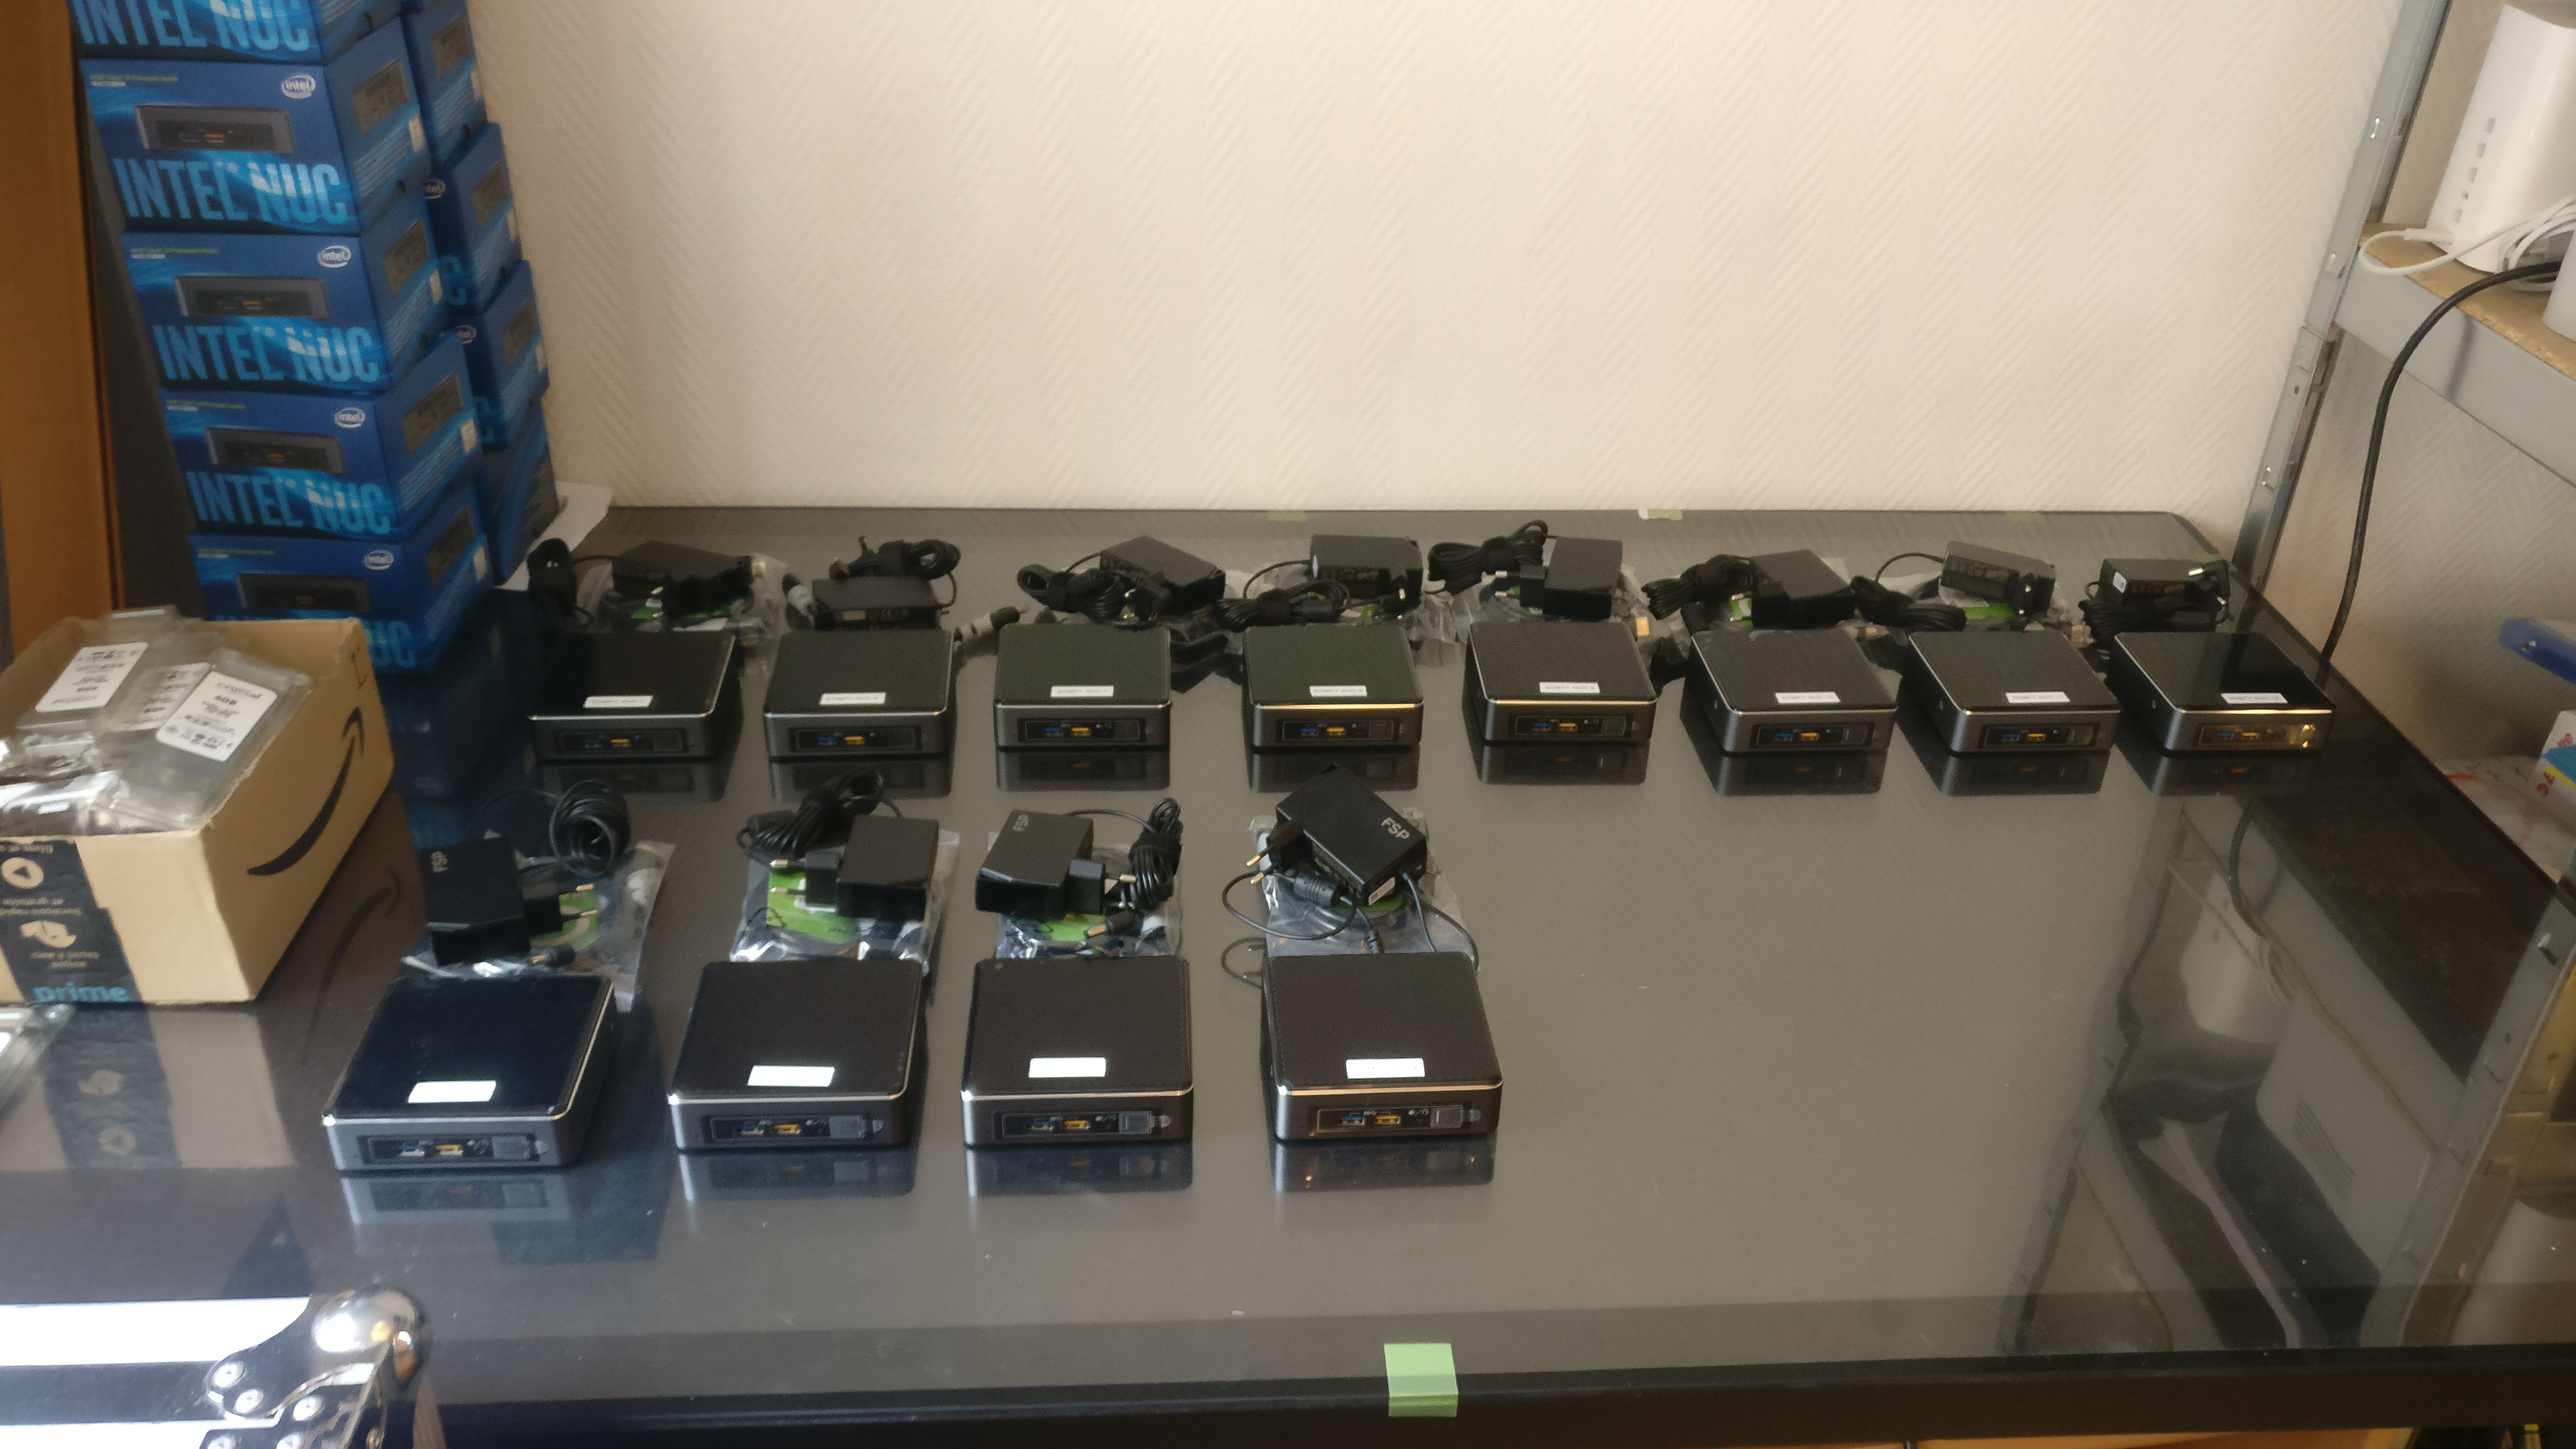
\includegraphics[scale=0.4]{img/somfy-nuc.jpg}
    \caption{Les 12 NUC hébergeant l'application de présentation}
\end{figure}

J'ai donc installé le système sur une machine que l'on appellera master.
J'ai ensuite utilisé CloneZilla pour faire une image du disque de cette machine et pouvoir la répliquer.

Après l'installation, nous avons trouvé quelques problèmes qui devaient être corrigés.
N'ayant pas le temps de réinstaller un clone sur toutes les machines, nous avons mis en réseau toutes les machines.
Il suffit alors d'utiliser \texttt{cssh} pour effectuer les mêmes actions en synchronisé sur toutes les machines.
\texttt{cssh} est un utilitaire permettant de créer un certain nombre de terminaux ssh tous synchronisés;
Il est alors aisé d'administrer un ensemble de machines en même temps.

\begin{figure}[h]
    \centering
    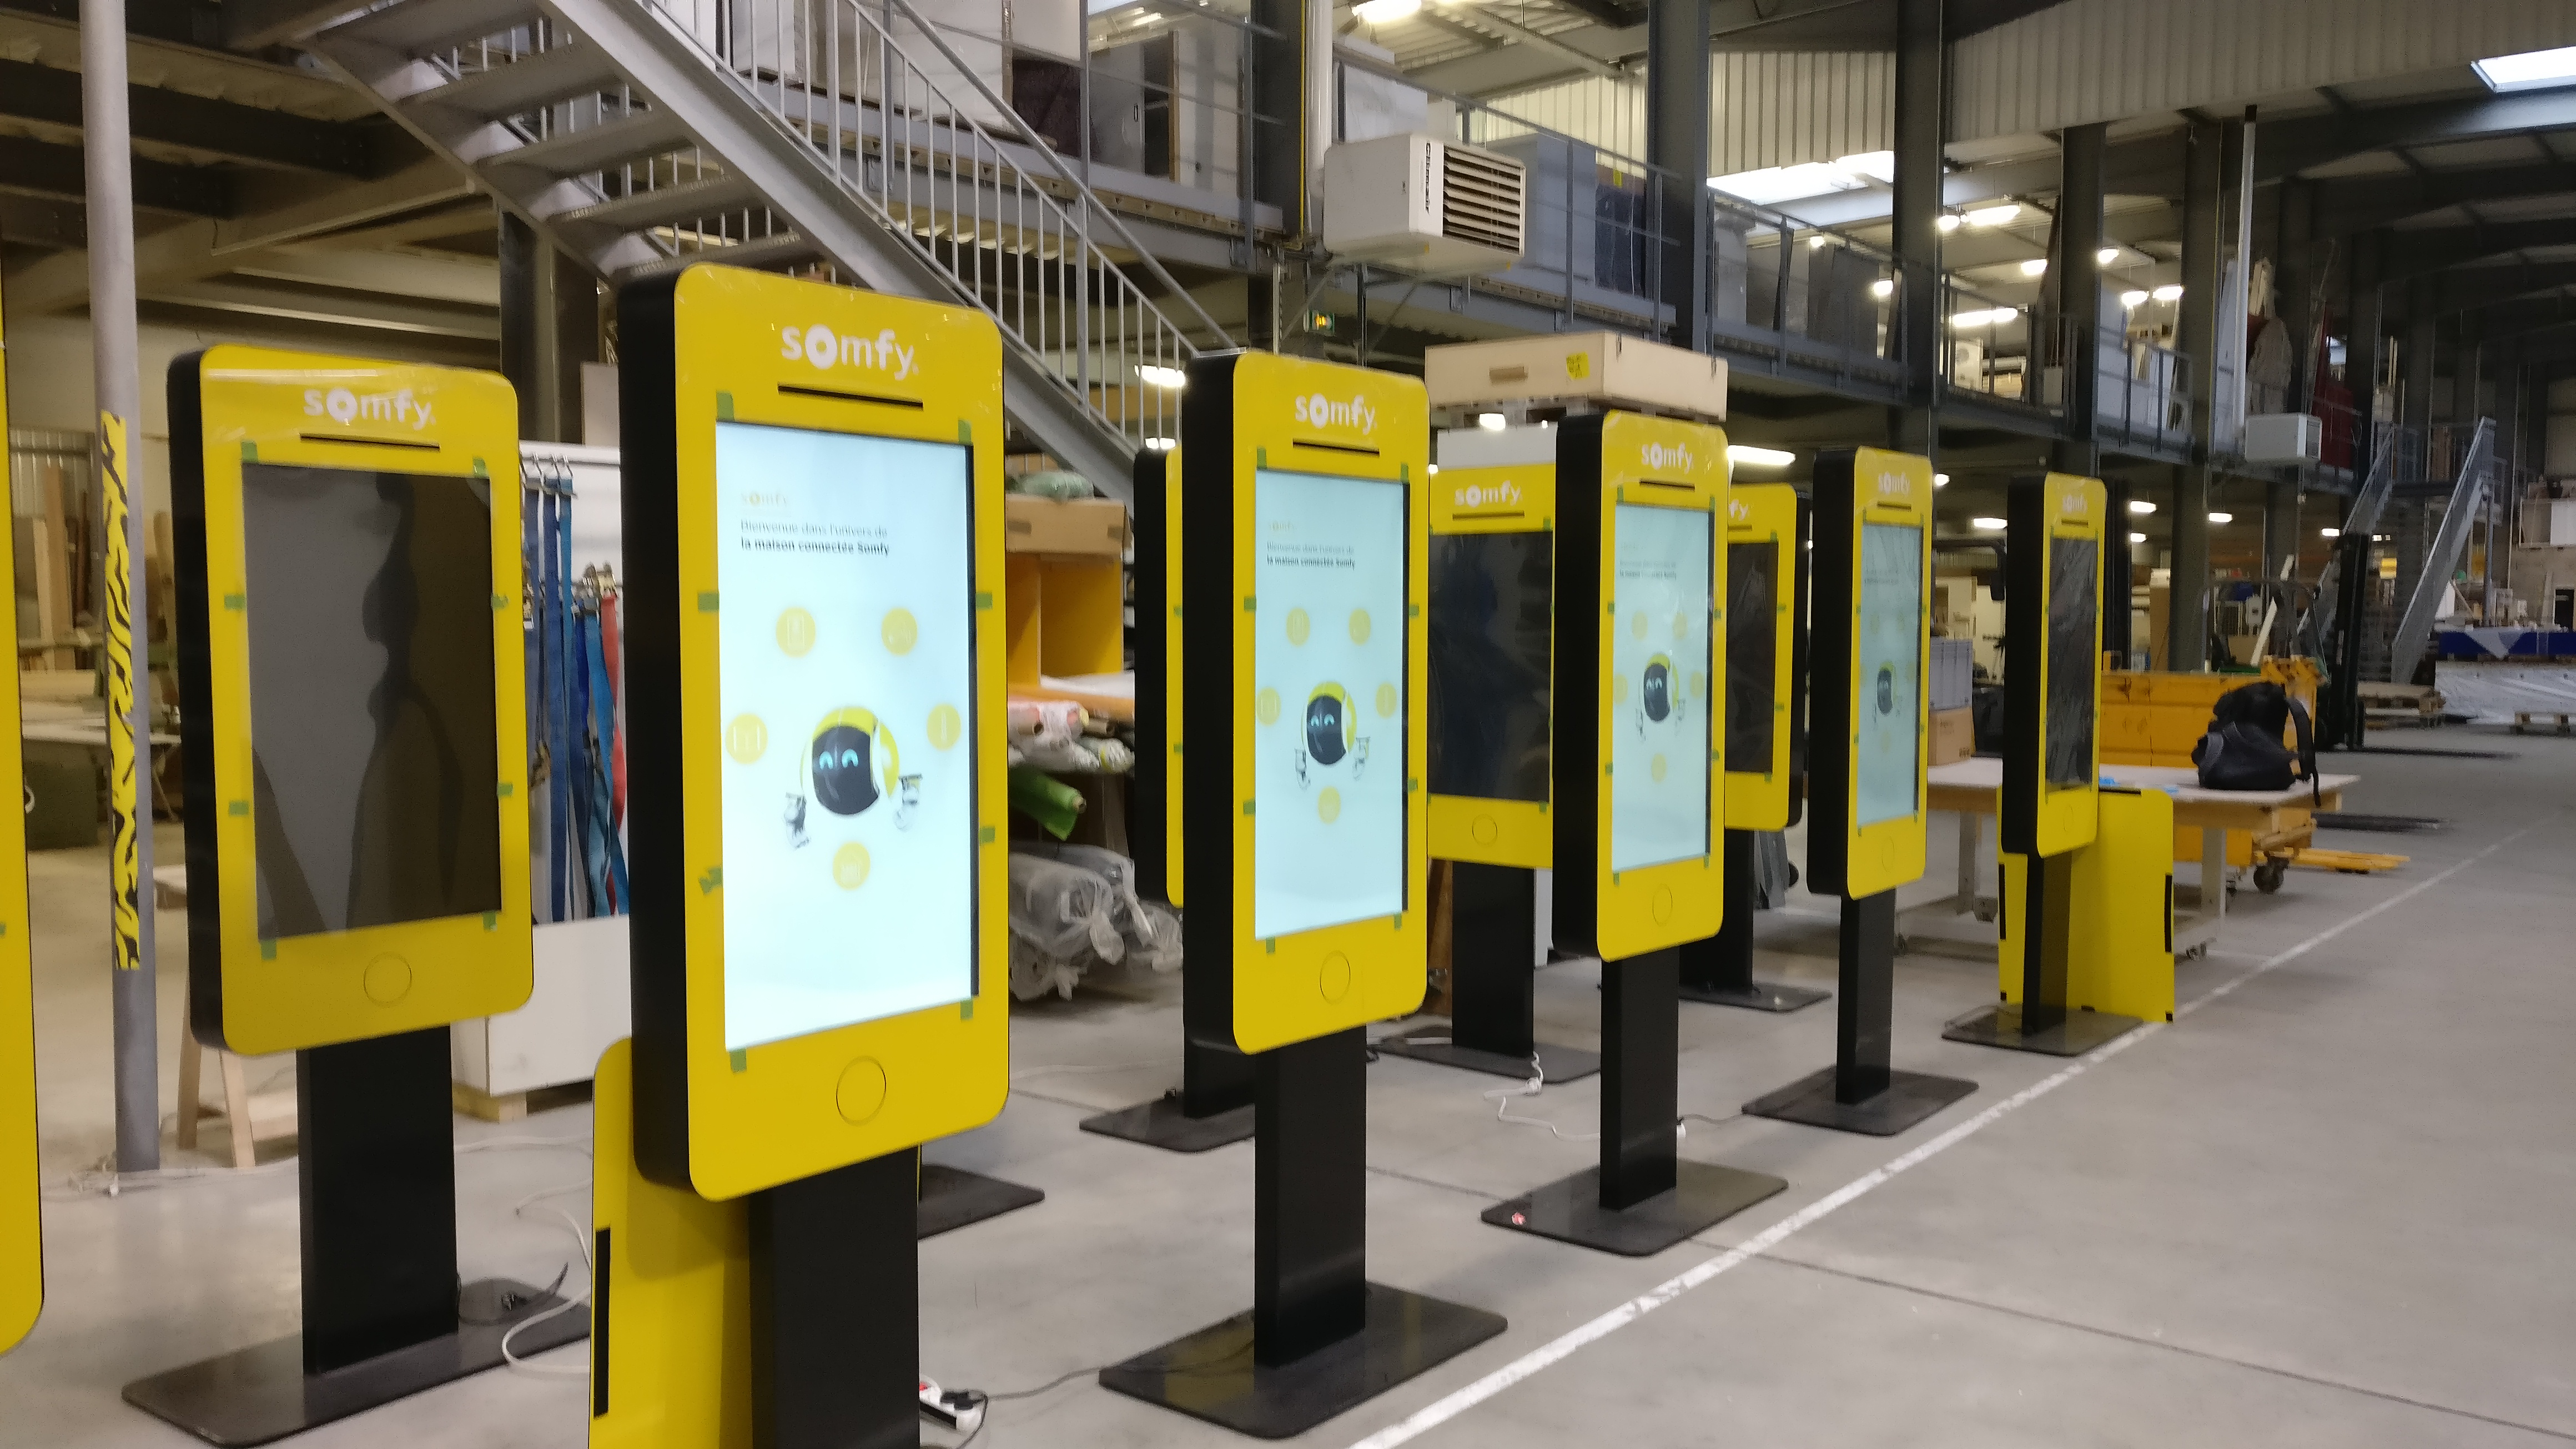
\includegraphics[scale=0.4]{img/somfy-install.jpg}
    \caption{Bornes Somfy lors de l'installation des machines dans leurs habitacles}
\end{figure}

\subsection{Conclusion}

Ce projet fut intéressant, car il m'a permis de me plonger plus en profondeur sur les composants d'un système Linux pour contrôler son fonctionnement.
Malgré la grande partie de recherche pour dégager la meilleure solution, j'ai quand même eu l'occasion de travailler sur un système de mise à jour innovant.
Le projet est à présent terminé et les bornes ont été disposées dans les magasins vendant la technologie Somfy.
